\section{Auswertung}
\label{sec:Auswertung}

\subsection{Ablenkung im elektrischen Feld}

\begin{table}
	\caption{Efeld amk.}
	\label{tab:efeldtab}
	\centering
	\begin{tabular}{cccc}
	\toprule
		& & $U_{\mathrm{d}}$ für & \\
		\midrule
		$D$ / \si{\centi\meter} & $U_{\mathrm{b}}=\SI{400}{\volt}$ & $U_{\mathrm{b}}=\SI{300}{\volt}$ & $U_{\mathrm{b}}=\SI{400}{\volt}$ \\
		\midrule
		0.000 & -7.70 & -8.2 & -6.0 \\
		0.635 & -5.40 & -5.4 & -4.3 \\
		1.270 & -1.72 & -1.5 & -1.6 \\
		1.905 & 5.62 & 3.1 & 0.9 \\
		2.540 & 9.00 & 5.4 & 3.1 \\
		3.175 & 14.95 & 9.5 & 5.4 \\
		3.810 & 22.60 & 14.2 & 8.4 \\
		4.445 & 28.40 & 19.1 & 11.5 \\
		5.080 & 33.00 & 23.5 & 14.0 \\
	\bottomrule
	\end{tabular}
\end{table}

\begin{table}
	\caption{Bestimmte Synchronisationsfrequenzen zur Erzeugung von stehenden Wellen auf dem Schirm.}
	\label{tab:saegen}
	\centering
	\begin{tabular}{cc}
	\toprule
		Frequenzverhältnis $n$ & $\nu$ / $\si{\hertz}$ \\
	\midrule
		0.5 & 39.96 \\
		1.0 & 79.95 \\
		2.0 & 159.85 \\
		3.0 & 239.73 \\
	\bottomrule
	\end{tabular}
\end{table}




%\begin{figure}
%  \centering
%  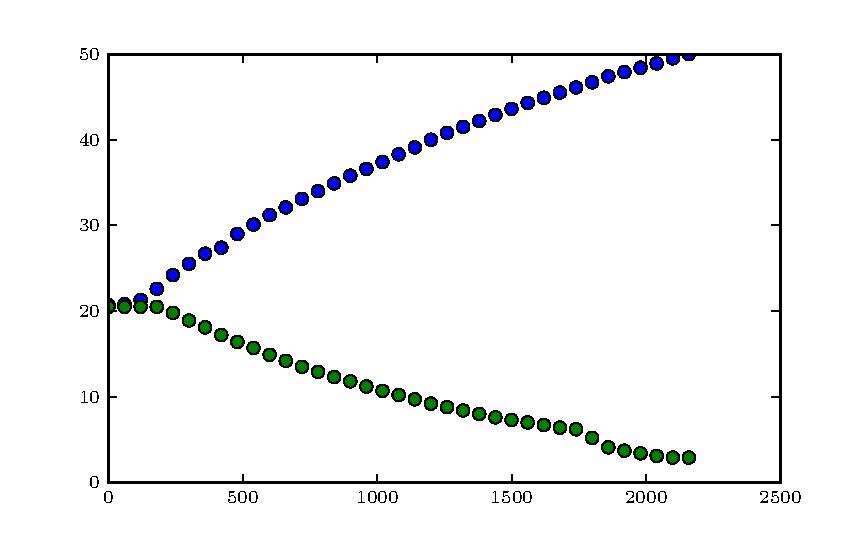
\includegraphics{plot.pdf}
%  \caption{Plot.}
%  \label{fig:plot}
%\end{figure}

%%%%%%%%%%%%%%%%%%%%%%%%%%%%%%%%%%%%%%%%%%%%%%%%%%%%%%%%%%%%%%%%%%%%%%%%%%%%%%%%%%%%%%%%%%%
\FloatBarrier
\subsection{Ablenkung im magnetischen Feld}

\subsubsection{Bestimmung von $\frac{\symup{e}_0}{\symup{m}_0}$}
Die Messergebnisse zur Berechnung von $\frac{\symup{e}_0}{\symup{m}_0}$ sind in Tabelle
\ref{tab:efeldtab} aufgetragen. Es wird eine lineare Ausgleichsrechnung der Form 
\begin{equation*}
	y = m \cdot x + b
\end{equation*}
gemäß Formel \eqref{eqn:???} mit scipy/python \cite{scipy} durchgeführt. Hierbei entspricht das
$y$ dem Faktor $\frac{D}{L^2+D^2}$ und das $x$ der Flussdichte $B$.
Die Paramter ergeben sich zu
m = b =  \begin{gather*}
	m = -\SI{15548(3386)}{\kelvin} \mathrm{,} \\
	b = \SI{2.6(3)}{\per\meter} \mathrm{.}
\end{gather*}
\begin{figure}
  \centering
  \includegraphics{Messdaten/plotbfeld.pdf}
  \caption{Plot.}
  \label{fig:bfeldplot}
\end{figure}
Die Ausgleichsgerade mit den Messwerten ist in Abbildung \ref{fig:bfeldplot} dargestellt.

\begin{table}
	\caption{Messwerte für die Verschiebung $D$ in Abhängigkeit von Strom blavla..}
	\label{tab:bfeldtab}
	\centering
	\begin{tabular}{ccc}
	\toprule
		$D$ / $\si{\centi\meter}$ & $I$ / $\si{\ampere}$ bei $U_{\mathrm{b}}=\SI{250}{\volt}$ & $I$ / $\si{\ampere}$ bei $U_{\mathrm{b}}=\SI{450}{\volt}$ \\
	\midrule
		0.635 & 0.35 & 0.46 \\
		1.270 & 0.67 & 0.83 \\
		1.905 & 0.98 & 1.26 \\
		2.540 & 1.21 & 1.69 \\
		3.175 & 1.57 & 2.09 \\
		3.810 & 1.90 & 2.52 \\
		4.445 & 2.21 & 2.94 \\
		5.080 & 2.53 & - \\
	\bottomrule
	\end{tabular}
\end{table}
